% Created by tikzDevice version 0.12.3 on 2019-09-02 17:59:43
% !TEX encoding = UTF-8 Unicode
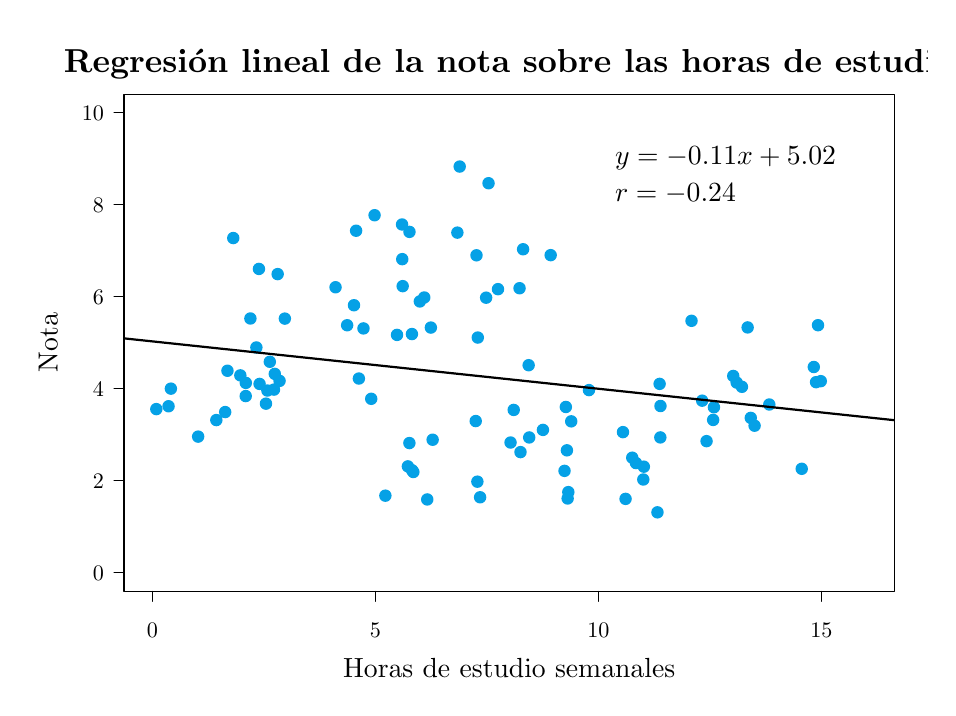
\begin{tikzpicture}[x=1pt,y=1pt]
\definecolor{fillColor}{RGB}{255,255,255}
\path[use as bounding box,fill=fillColor,fill opacity=0.00] (0,0) rectangle (325.21,238.49);
\begin{scope}
\path[clip] ( 34.80, 34.80) rectangle (313.21,214.49);
\definecolor{fillColor}{RGB}{5,161,230}

\path[fill=fillColor] ( 61.60, 90.72) circle (  2.25);

\path[fill=fillColor] (135.35,154.84) circle (  2.25);

\path[fill=fillColor] (133.46,127.47) circle (  2.25);

\path[fill=fillColor] (135.51,145.09) circle (  2.25);

\path[fill=fillColor] (169.95,144.00) circle (  2.25);

\path[fill=fillColor] (137.96,164.70) circle (  2.25);

\path[fill=fillColor] ( 46.49,100.66) circle (  2.25);

\path[fill=fillColor] ( 78.83,110.13) circle (  2.25);

\path[fill=fillColor] (141.70,139.56) circle (  2.25);

\path[fill=fillColor] (119.68,111.70) circle (  2.25);

\path[fill=fillColor] (145.69,130.12) circle (  2.25);

\path[fill=fillColor] (124.14,104.38) circle (  2.25);

\path[fill=fillColor] ( 86.11,102.63) circle (  2.25);

\path[fill=fillColor] (179.02,158.42) circle (  2.25);

\path[fill=fillColor] ( 87.50,117.76) circle (  2.25);

\path[fill=fillColor] (166.53,182.28) circle (  2.25);

\path[fill=fillColor] ( 86.62,107.37) circle (  2.25);

\path[fill=fillColor] ( 83.80,109.76) circle (  2.25);

\path[fill=fillColor] ( 72.19,114.52) circle (  2.25);

\path[fill=fillColor] ( 78.79,105.37) circle (  2.25);

\path[fill=fillColor] ( 91.02,110.86) circle (  2.25);

\path[fill=fillColor] ( 89.00,107.71) circle (  2.25);

\path[fill=fillColor] ( 68.17, 96.70) circle (  2.25);

\path[fill=fillColor] ( 50.91,101.69) circle (  2.25);

\path[fill=fillColor] ( 76.84,112.85) circle (  2.25);

\path[fill=fillColor] (162.65,126.51) circle (  2.25);

\path[fill=fillColor] (121.34,129.81) circle (  2.25);

\path[fill=fillColor] (177.74,144.34) circle (  2.25);

\path[fill=fillColor] (165.66,140.92) circle (  2.25);

\path[fill=fillColor] ( 51.75,108.05) circle (  2.25);

\path[fill=fillColor] (111.25,144.69) circle (  2.25);

\path[fill=fillColor] ( 83.57,151.31) circle (  2.25);

\path[fill=fillColor] ( 89.29,113.39) circle (  2.25);

\path[fill=fillColor] (118.68,165.11) circle (  2.25);

\path[fill=fillColor] ( 71.37, 99.59) circle (  2.25);

\path[fill=fillColor] (155.27,164.43) circle (  2.25);

\path[fill=fillColor] ( 74.29,162.47) circle (  2.25);

\path[fill=fillColor] ( 82.64,122.93) circle (  2.25);

\path[fill=fillColor] (188.98,156.29) circle (  2.25);

\path[fill=fillColor] (162.18,156.24) circle (  2.25);

\path[fill=fillColor] (125.35,170.72) circle (  2.25);

\path[fill=fillColor] (138.85,127.78) circle (  2.25);

\path[fill=fillColor] ( 90.33,149.44) circle (  2.25);

\path[fill=fillColor] (135.28,167.37) circle (  2.25);

\path[fill=fillColor] ( 92.93,133.36) circle (  2.25);

\path[fill=fillColor] (117.91,138.19) circle (  2.25);

\path[fill=fillColor] (143.30,140.99) circle (  2.25);

\path[fill=fillColor] (115.44,130.96) circle (  2.25);

\path[fill=fillColor] ( 80.48,133.40) circle (  2.25);

\path[fill=fillColor] (156.11,188.30) circle (  2.25);

\path[fill=fillColor] (196.41, 96.24) circle (  2.25);

\path[fill=fillColor] (162.50, 74.44) circle (  2.25);

\path[fill=fillColor] (138.91, 78.56) circle (  2.25);

\path[fill=fillColor] (262.67, 94.66) circle (  2.25);

\path[fill=fillColor] (163.48, 68.80) circle (  2.25);

\path[fill=fillColor] (284.88,110.39) circle (  2.25);

\path[fill=fillColor] (222.65, 79.85) circle (  2.25);

\path[fill=fillColor] (286.59,110.76) circle (  2.25);

\path[fill=fillColor] (186.19, 93.14) circle (  2.25);

\path[fill=fillColor] (215.11, 92.34) circle (  2.25);

\path[fill=fillColor] (194.86, 85.76) circle (  2.25);

\path[fill=fillColor] (218.46, 83.10) circle (  2.25);

\path[fill=fillColor] (195.36, 70.66) circle (  2.25);

\path[fill=fillColor] (161.90, 96.34) circle (  2.25);

\path[fill=fillColor] (139.36, 77.93) circle (  2.25);

\path[fill=fillColor] (228.35,109.77) circle (  2.25);

\path[fill=fillColor] (195.12, 68.37) circle (  2.25);

\path[fill=fillColor] (137.39, 79.96) circle (  2.25);

\path[fill=fillColor] (254.95,112.63) circle (  2.25);

\path[fill=fillColor] (178.08, 85.12) circle (  2.25);

\path[fill=fillColor] (247.69, 96.75) circle (  2.25);

\path[fill=fillColor] (219.81, 81.16) circle (  2.25);

\path[fill=fillColor] (239.88,132.56) circle (  2.25);

\path[fill=fillColor] (194.47,101.43) circle (  2.25);

\path[fill=fillColor] (181.03,116.52) circle (  2.25);

\path[fill=fillColor] (247.98,101.32) circle (  2.25);

\path[fill=fillColor] (193.99, 78.34) circle (  2.25);

\path[fill=fillColor] (216.04, 68.22) circle (  2.25);

\path[fill=fillColor] (144.38, 68.01) circle (  2.25);

\path[fill=fillColor] (174.49, 88.58) circle (  2.25);

\path[fill=fillColor] (202.82,107.53) circle (  2.25);

\path[fill=fillColor] (181.23, 90.41) circle (  2.25);

\path[fill=fillColor] (222.46, 75.22) circle (  2.25);

\path[fill=fillColor] (137.93, 88.39) circle (  2.25);

\path[fill=fillColor] (279.70, 79.09) circle (  2.25);

\path[fill=fillColor] (129.25, 69.38) circle (  2.25);

\path[fill=fillColor] (261.29, 97.48) circle (  2.25);

\path[fill=fillColor] (227.57, 63.36) circle (  2.25);

\path[fill=fillColor] (175.63,100.36) circle (  2.25);

\path[fill=fillColor] (245.31, 89.08) circle (  2.25);

\path[fill=fillColor] (228.61, 90.43) circle (  2.25);

\path[fill=fillColor] (285.59,130.97) circle (  2.25);

\path[fill=fillColor] (146.34, 89.59) circle (  2.25);

\path[fill=fillColor] (267.98,102.32) circle (  2.25);

\path[fill=fillColor] (256.19,110.24) circle (  2.25);

\path[fill=fillColor] (258.09,108.72) circle (  2.25);

\path[fill=fillColor] (260.16,130.17) circle (  2.25);

\path[fill=fillColor] (243.73,103.70) circle (  2.25);

\path[fill=fillColor] (284.06,115.87) circle (  2.25);

\path[fill=fillColor] (228.66,101.78) circle (  2.25);
\end{scope}
\begin{scope}
\path[clip] (  0.00,  0.00) rectangle (325.21,238.49);
\definecolor{drawColor}{RGB}{0,0,0}

\path[draw=drawColor,line width= 0.4pt,line join=round,line cap=round] ( 45.11, 34.80) -- (286.79, 34.80);

\path[draw=drawColor,line width= 0.4pt,line join=round,line cap=round] ( 45.11, 34.80) -- ( 45.11, 31.21);

\path[draw=drawColor,line width= 0.4pt,line join=round,line cap=round] (125.67, 34.80) -- (125.67, 31.21);

\path[draw=drawColor,line width= 0.4pt,line join=round,line cap=round] (206.23, 34.80) -- (206.23, 31.21);

\path[draw=drawColor,line width= 0.4pt,line join=round,line cap=round] (286.79, 34.80) -- (286.79, 31.21);

\node[text=drawColor,anchor=base,inner sep=0pt, outer sep=0pt, scale=  0.80] at ( 45.11, 18.00) {0};

\node[text=drawColor,anchor=base,inner sep=0pt, outer sep=0pt, scale=  0.80] at (125.67, 18.00) {5};

\node[text=drawColor,anchor=base,inner sep=0pt, outer sep=0pt, scale=  0.80] at (206.23, 18.00) {10};

\node[text=drawColor,anchor=base,inner sep=0pt, outer sep=0pt, scale=  0.80] at (286.79, 18.00) {15};

\path[draw=drawColor,line width= 0.4pt,line join=round,line cap=round] ( 34.80, 41.46) -- ( 34.80,207.84);

\path[draw=drawColor,line width= 0.4pt,line join=round,line cap=round] ( 34.80, 41.46) -- ( 31.21, 41.46);

\path[draw=drawColor,line width= 0.4pt,line join=round,line cap=round] ( 34.80, 74.73) -- ( 31.21, 74.73);

\path[draw=drawColor,line width= 0.4pt,line join=round,line cap=round] ( 34.80,108.01) -- ( 31.21,108.01);

\path[draw=drawColor,line width= 0.4pt,line join=round,line cap=round] ( 34.80,141.28) -- ( 31.21,141.28);

\path[draw=drawColor,line width= 0.4pt,line join=round,line cap=round] ( 34.80,174.56) -- ( 31.21,174.56);

\path[draw=drawColor,line width= 0.4pt,line join=round,line cap=round] ( 34.80,207.84) -- ( 31.21,207.84);

\node[text=drawColor,anchor=base east,inner sep=0pt, outer sep=0pt, scale=  0.80] at ( 27.60, 38.70) {0};

\node[text=drawColor,anchor=base east,inner sep=0pt, outer sep=0pt, scale=  0.80] at ( 27.60, 71.98) {2};

\node[text=drawColor,anchor=base east,inner sep=0pt, outer sep=0pt, scale=  0.80] at ( 27.60,105.25) {4};

\node[text=drawColor,anchor=base east,inner sep=0pt, outer sep=0pt, scale=  0.80] at ( 27.60,138.53) {6};

\node[text=drawColor,anchor=base east,inner sep=0pt, outer sep=0pt, scale=  0.80] at ( 27.60,171.80) {8};

\node[text=drawColor,anchor=base east,inner sep=0pt, outer sep=0pt, scale=  0.80] at ( 27.60,205.08) {10};

\path[draw=drawColor,line width= 0.4pt,line join=round,line cap=round] ( 34.80, 34.80) --
	(313.21, 34.80) --
	(313.21,214.49) --
	( 34.80,214.49) --
	( 34.80, 34.80);
\end{scope}
\begin{scope}
\path[clip] (  0.00,  0.00) rectangle (325.21,238.49);
\definecolor{drawColor}{RGB}{0,0,0}

\node[text=drawColor,anchor=base,inner sep=0pt, outer sep=0pt, scale=  1.20] at (174.01,222.30) {\bfseries Regresión lineal de la nota sobre las horas de estudio};

\node[text=drawColor,anchor=base,inner sep=0pt, outer sep=0pt, scale=  1.00] at (174.01,  3.60) {Horas de estudio semanales};

\node[text=drawColor,rotate= 90.00,anchor=base,inner sep=0pt, outer sep=0pt, scale=  1.00] at ( 10.80,124.65) {Nota};
\end{scope}
\begin{scope}
\path[clip] ( 34.80, 34.80) rectangle (313.21,214.49);
\definecolor{drawColor}{RGB}{0,0,0}

\path[draw=drawColor,line width= 0.8pt,line join=round,line cap=round] ( 34.80,126.22) -- (313.21, 96.65);

\node[text=drawColor,anchor=base west,inner sep=0pt, outer sep=0pt, scale=  1.00] at (212.23,188.90) {$y= -0.11 x + 5.02 $};

\node[text=drawColor,anchor=base west,inner sep=0pt, outer sep=0pt, scale=  1.00] at (212.23,175.59) {$r= -0.24 $};
\end{scope}
\end{tikzpicture}
